\documentclass[1p]{elsarticle_modified}
%\bibliographystyle{elsarticle-num}

%\usepackage[colorlinks]{hyperref}
%\usepackage{abbrmath_seonhwa} %\Abb, \Ascr, \Acal ,\Abf, \Afrak
\usepackage{amsfonts}
\usepackage{amssymb}
\usepackage{amsmath}
\usepackage{amsthm}
\usepackage{scalefnt}
\usepackage{amsbsy}
\usepackage{kotex}
\usepackage{caption}
\usepackage{subfig}
\usepackage{color}
\usepackage{graphicx}
\usepackage{xcolor} %% white, black, red, green, blue, cyan, magenta, yellow
\usepackage{float}
\usepackage{setspace}
\usepackage{hyperref}

\usepackage{tikz}
\usetikzlibrary{arrows}

\usepackage{multirow}
\usepackage{array} % fixed length table
\usepackage{hhline}

%%%%%%%%%%%%%%%%%%%%%
\makeatletter
\renewcommand*\env@matrix[1][\arraystretch]{%
	\edef\arraystretch{#1}%
	\hskip -\arraycolsep
	\let\@ifnextchar\new@ifnextchar
	\array{*\c@MaxMatrixCols c}}
\makeatother %https://tex.stackexchange.com/questions/14071/how-can-i-increase-the-line-spacing-in-a-matrix
%%%%%%%%%%%%%%%

\usepackage[normalem]{ulem}

\newcommand{\msout}[1]{\ifmmode\text{\sout{\ensuremath{#1}}}\else\sout{#1}\fi}
%SOURCE: \msout is \stkout macro in https://tex.stackexchange.com/questions/20609/strikeout-in-math-mode

\newcommand{\cancel}[1]{
	\ifmmode
	{\color{red}\msout{#1}}
	\else
	{\color{red}\sout{#1}}
	\fi
}

\newcommand{\add}[1]{
	{\color{blue}\uwave{#1}}
}

\newcommand{\replace}[2]{
	\ifmmode
	{\color{red}\msout{#1}}{\color{blue}\uwave{#2}}
	\else
	{\color{red}\sout{#1}}{\color{blue}\uwave{#2}}
	\fi
}

\newcommand{\Sol}{\mathcal{S}} %segment
\newcommand{\D}{D} %diagram
\newcommand{\A}{\mathcal{A}} %arc


%%%%%%%%%%%%%%%%%%%%%%%%%%%%%5 test

\def\sl{\operatorname{\textup{SL}}(2,\Cbb)}
\def\psl{\operatorname{\textup{PSL}}(2,\Cbb)}
\def\quan{\mkern 1mu \triangleright \mkern 1mu}

\theoremstyle{definition}
\newtheorem{thm}{Theorem}[section]
\newtheorem{prop}[thm]{Proposition}
\newtheorem{lem}[thm]{Lemma}
\newtheorem{ques}[thm]{Question}
\newtheorem{cor}[thm]{Corollary}
\newtheorem{defn}[thm]{Definition}
\newtheorem{exam}[thm]{Example}
\newtheorem{rmk}[thm]{Remark}
\newtheorem{alg}[thm]{Algorithm}

\newcommand{\I}{\sqrt{-1}}
\begin{document}

%\begin{frontmatter}
%
%\title{Boundary parabolic representations of knots up to 8 crossings}
%
%%% Group authors per affiliation:
%\author{Yunhi Cho} 
%\address{Department of Mathematics, University of Seoul, Seoul, Korea}
%\ead{yhcho@uos.ac.kr}
%
%
%\author{Seonhwa Kim} %\fnref{s_kim}}
%\address{Center for Geometry and Physics, Institute for Basic Science, Pohang, 37673, Korea}
%\ead{ryeona17@ibs.re.kr}
%
%\author{Hyuk Kim}
%\address{Department of Mathematical Sciences, Seoul National University, Seoul 08826, Korea}
%\ead{hyukkim@snu.ac.kr}
%
%\author{Seokbeom Yoon}
%\address{Department of Mathematical Sciences, Seoul National University, Seoul, 08826,  Korea}
%\ead{sbyoon15@snu.ac.kr}
%
%\begin{abstract}
%We find all boundary parabolic representation of knots up to 8 crossings.
%
%\end{abstract}
%\begin{keyword}
%    \MSC[2010] 57M25 
%\end{keyword}
%
%\end{frontmatter}

%\linenumbers
%\tableofcontents
%
\newcommand\colored[1]{\textcolor{white}{\rule[-0.35ex]{0.8em}{1.4ex}}\kern-0.8em\color{red} #1}%
%\newcommand\colored[1]{\textcolor{white}{ #1}\kern-2.17ex	\textcolor{white}{ #1}\kern-1.81ex	\textcolor{white}{ #1}\kern-2.15ex\color{red}#1	}

{\Large $\underline{12a_{0469}~(K12a_{0469})}$}

\setlength{\tabcolsep}{10pt}
\renewcommand{\arraystretch}{1.6}
\vspace{1cm}\begin{tabular}{m{100pt}>{\centering\arraybackslash}m{274pt}}
\multirow{5}{120pt}{
	\centering
	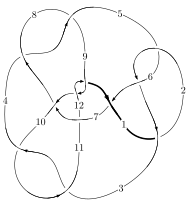
\includegraphics[width=112pt]{../../../GIT/diagram.site/Diagrams/png/1270_12a_0469.png}\\
\ \ \ A knot diagram\footnotemark}&
\allowdisplaybreaks
\textbf{Linearized knot diagam} \\
\cline{2-2}
 &
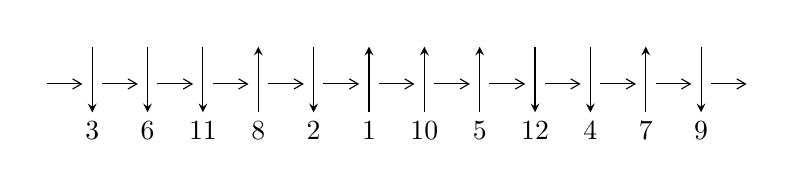
\begin{tikzpicture}[x=20pt, y=17pt]
	% nodes
	\node (C0) at (0, 0) {};
	\node (C1) at (1, 0) {};
	\node (C1U) at (1, +1) {};
	\node (C1D) at (1, -1) {3};

	\node (C2) at (2, 0) {};
	\node (C2U) at (2, +1) {};
	\node (C2D) at (2, -1) {6};

	\node (C3) at (3, 0) {};
	\node (C3U) at (3, +1) {};
	\node (C3D) at (3, -1) {11};

	\node (C4) at (4, 0) {};
	\node (C4U) at (4, +1) {};
	\node (C4D) at (4, -1) {8};

	\node (C5) at (5, 0) {};
	\node (C5U) at (5, +1) {};
	\node (C5D) at (5, -1) {2};

	\node (C6) at (6, 0) {};
	\node (C6U) at (6, +1) {};
	\node (C6D) at (6, -1) {1};

	\node (C7) at (7, 0) {};
	\node (C7U) at (7, +1) {};
	\node (C7D) at (7, -1) {10};

	\node (C8) at (8, 0) {};
	\node (C8U) at (8, +1) {};
	\node (C8D) at (8, -1) {5};

	\node (C9) at (9, 0) {};
	\node (C9U) at (9, +1) {};
	\node (C9D) at (9, -1) {12};

	\node (C10) at (10, 0) {};
	\node (C10U) at (10, +1) {};
	\node (C10D) at (10, -1) {4};

	\node (C11) at (11, 0) {};
	\node (C11U) at (11, +1) {};
	\node (C11D) at (11, -1) {7};

	\node (C12) at (12, 0) {};
	\node (C12U) at (12, +1) {};
	\node (C12D) at (12, -1) {9};
	\node (C13) at (13, 0) {};

	% arrows
	\draw[->,>={angle 60}]
	(C0) edge (C1) (C1) edge (C2) (C2) edge (C3) (C3) edge (C4) (C4) edge (C5) (C5) edge (C6) (C6) edge (C7) (C7) edge (C8) (C8) edge (C9) (C9) edge (C10) (C10) edge (C11) (C11) edge (C12) (C12) edge (C13) ;	\draw[->,>=stealth]
	(C1U) edge (C1D) (C2U) edge (C2D) (C3U) edge (C3D) (C4D) edge (C4U) (C5U) edge (C5D) (C6D) edge (C6U) (C7D) edge (C7U) (C8D) edge (C8U) (C9U) edge (C9D) (C10U) edge (C10D) (C11D) edge (C11U) (C12U) edge (C12D) ;
	\end{tikzpicture} \\
\hhline{~~} \\& 
\textbf{Solving Sequence} \\ \cline{2-2} 
 &
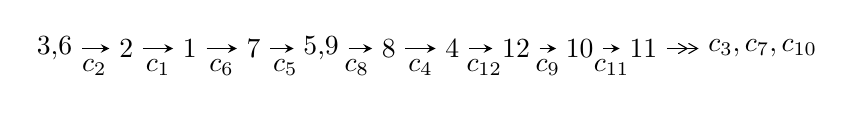
\begin{tikzpicture}[x=23pt, y=7pt]
	% node
	\node (A0) at (-1/8, 0) {3,6};
	\node (A1) at (1, 0) {2};
	\node (A2) at (2, 0) {1};
	\node (A3) at (3, 0) {7};
	\node (A4) at (65/16, 0) {5,9};
	\node (A5) at (41/8, 0) {8};
	\node (A6) at (49/8, 0) {4};
	\node (A7) at (57/8, 0) {12};
	\node (A8) at (65/8, 0) {10};
	\node (A9) at (73/8, 0) {11};
	\node (C1) at (1/2, -1) {$c_{2}$};
	\node (C2) at (3/2, -1) {$c_{1}$};
	\node (C3) at (5/2, -1) {$c_{6}$};
	\node (C4) at (7/2, -1) {$c_{5}$};
	\node (C5) at (37/8, -1) {$c_{8}$};
	\node (C6) at (45/8, -1) {$c_{4}$};
	\node (C7) at (53/8, -1) {$c_{12}$};
	\node (C8) at (61/8, -1) {$c_{9}$};
	\node (C9) at (69/8, -1) {$c_{11}$};
	\node (A10) at (11, 0) {$c_{3},c_{7},c_{10}$};

	% edge
	\draw[->,>=stealth]	
	(A0) edge (A1) (A1) edge (A2) (A2) edge (A3) (A3) edge (A4) (A4) edge (A5) (A5) edge (A6) (A6) edge (A7) (A7) edge (A8) (A8) edge (A9) ;
	\draw[->>,>={angle 60}]	
	(A9) edge (A10);
\end{tikzpicture} \\ 

\end{tabular} \\

\footnotetext{
The image of knot diagram is generated by the software ``\textbf{Draw programme}" developed by Andrew Bartholomew(\url{http://www.layer8.co.uk/maths/draw/index.htm\#Running-draw}), where we modified some parts for our purpose(\url{https://github.com/CATsTAILs/LinksPainter}).
}\phantom \\ \newline 
\centering \textbf{Ideals for irreducible components\footnotemark of $X_{\text{par}}$} 
 
\begin{align*}
I^u_{1}&=\langle 
6.63633\times10^{186} u^{142}+2.53542\times10^{189} u^{141}+\cdots+9.01034\times10^{189} b+3.59708\times10^{190},\\
\phantom{I^u_{1}}&\phantom{= \langle  }-8.67414\times10^{190} u^{142}+3.49780\times10^{191} u^{141}+\cdots+4.23486\times10^{191} a-1.16899\times10^{193},\\
\phantom{I^u_{1}}&\phantom{= \langle  }u^{143}-3 u^{142}+\cdots+110 u-47\rangle \\
I^u_{2}&=\langle 
4 u^{34}+7 u^{33}+\cdots+b-5,\;-3 u^{34}-2 u^{33}+\cdots+a+2,\;u^{35}+2 u^{34}+\cdots-2 u-1\rangle \\
\\
\end{align*}
\raggedright * 2 irreducible components of $\dim_{\mathbb{C}}=0$, with total 178 representations.\\
\footnotetext{All coefficients of polynomials are rational numbers. But the coefficients are sometimes approximated in decimal forms when there is not enough margin.}
\newpage
\renewcommand{\arraystretch}{1}
\centering \section*{I. $I^u_{1}= \langle 6.64\times10^{186} u^{142}+2.54\times10^{189} u^{141}+\cdots+9.01\times10^{189} b+3.60\times10^{190},\;-8.67\times10^{190} u^{142}+3.50\times10^{191} u^{141}+\cdots+4.23\times10^{191} a-1.17\times10^{193},\;u^{143}-3 u^{142}+\cdots+110 u-47 \rangle$}
\flushleft \textbf{(i) Arc colorings}\\
\begin{tabular}{m{7pt} m{180pt} m{7pt} m{180pt} }
\flushright $a_{3}=$&$\begin{pmatrix}1\\0\end{pmatrix}$ \\
\flushright $a_{6}=$&$\begin{pmatrix}0\\u\end{pmatrix}$ \\
\flushright $a_{2}=$&$\begin{pmatrix}1\\- u^2\end{pmatrix}$ \\
\flushright $a_{1}=$&$\begin{pmatrix}- u^2+1\\- u^2\end{pmatrix}$ \\
\flushright $a_{7}=$&$\begin{pmatrix}u^5-2 u^3+u\\u^5- u^3+u\end{pmatrix}$ \\
\flushright $a_{5}=$&$\begin{pmatrix}u\\- u^3+u\end{pmatrix}$ \\
\flushright $a_{9}=$&$\begin{pmatrix}0.204827 u^{142}-0.825954 u^{141}+\cdots-44.4711 u+27.6040\\-0.000736524 u^{142}-0.281390 u^{141}+\cdots+8.40058 u-3.99217\end{pmatrix}$ \\
\flushright $a_{8}=$&$\begin{pmatrix}0.770473 u^{142}-2.27599 u^{141}+\cdots-96.6026 u+66.2237\\0.589171 u^{142}-1.10912 u^{141}+\cdots-43.1569 u+23.0231\end{pmatrix}$ \\
\flushright $a_{4}=$&$\begin{pmatrix}-0.623467 u^{142}+0.435106 u^{141}+\cdots+70.3674 u-10.6358\\0.402860 u^{142}-0.856118 u^{141}+\cdots-19.8741 u+12.8858\end{pmatrix}$ \\
\flushright $a_{12}=$&$\begin{pmatrix}-0.287141 u^{142}+0.974601 u^{141}+\cdots+31.1944 u-41.8783\\-1.17791 u^{142}+2.62231 u^{141}+\cdots+91.6207 u-54.4365\end{pmatrix}$ \\
\flushright $a_{10}=$&$\begin{pmatrix}-0.682533 u^{142}+1.81972 u^{141}+\cdots+86.3997 u-44.9083\\0.128085 u^{142}-0.345952 u^{141}+\cdots-14.7059 u+8.01038\end{pmatrix}$ \\
\flushright $a_{11}=$&$\begin{pmatrix}-1.00812 u^{142}+1.95993 u^{141}+\cdots+46.9184 u-61.1004\\-0.281878 u^{142}+0.435375 u^{141}+\cdots+17.4712 u-15.1734\end{pmatrix}$\\&\end{tabular}
\flushleft \textbf{(ii) Obstruction class $= -1$}\\~\\
\flushleft \textbf{(iii) Cusp Shapes $= -1.34172 u^{142}+2.00690 u^{141}+\cdots+81.0326 u-68.7918$}\\~\\
\newpage\renewcommand{\arraystretch}{1}
\flushleft \textbf{(iv) u-Polynomials at the component}\newline \\
\begin{tabular}{m{50pt}|m{274pt}}
Crossings & \hspace{64pt}u-Polynomials at each crossing \\
\hline $$\begin{aligned}c_{1}\end{aligned}$$&$\begin{aligned}
&u^{143}+69 u^{142}+\cdots+24038 u+2209
\end{aligned}$\\
\hline $$\begin{aligned}c_{2},c_{5}\end{aligned}$$&$\begin{aligned}
&u^{143}+3 u^{142}+\cdots+110 u+47
\end{aligned}$\\
\hline $$\begin{aligned}c_{3},c_{10}\end{aligned}$$&$\begin{aligned}
&u^{143}+2 u^{142}+\cdots+22312 u+8024
\end{aligned}$\\
\hline $$\begin{aligned}c_{4},c_{8}\end{aligned}$$&$\begin{aligned}
&u^{143}-60 u^{141}+\cdots+6466443 u+1229681
\end{aligned}$\\
\hline $$\begin{aligned}c_{6}\end{aligned}$$&$\begin{aligned}
&u^{143}+9 u^{142}+\cdots+1198600 u+745279
\end{aligned}$\\
\hline $$\begin{aligned}c_{7}\end{aligned}$$&$\begin{aligned}
&u^{143}+6 u^{142}+\cdots+586376963 u+10200841
\end{aligned}$\\
\hline $$\begin{aligned}c_{9},c_{12}\end{aligned}$$&$\begin{aligned}
&u^{143}-7 u^{142}+\cdots-220108 u+19079
\end{aligned}$\\
\hline $$\begin{aligned}c_{11}\end{aligned}$$&$\begin{aligned}
&u^{143}-2 u^{142}+\cdots+111690 u+3457
\end{aligned}$\\
\hline
\end{tabular}\\~\\
\newpage\renewcommand{\arraystretch}{1}
\flushleft \textbf{(v) Riley Polynomials at the component}\newline \\
\begin{tabular}{m{50pt}|m{274pt}}
Crossings & \hspace{64pt}Riley Polynomials at each crossing \\
\hline $$\begin{aligned}c_{1}\end{aligned}$$&$\begin{aligned}
&y^{143}+15 y^{142}+\cdots-116759262 y-4879681
\end{aligned}$\\
\hline $$\begin{aligned}c_{2},c_{5}\end{aligned}$$&$\begin{aligned}
&y^{143}-69 y^{142}+\cdots+24038 y-2209
\end{aligned}$\\
\hline $$\begin{aligned}c_{3},c_{10}\end{aligned}$$&$\begin{aligned}
&y^{143}+100 y^{142}+\cdots-1978348960 y-64384576
\end{aligned}$\\
\hline $$\begin{aligned}c_{4},c_{8}\end{aligned}$$&$\begin{aligned}
&y^{143}-120 y^{142}+\cdots+46027317196279 y-1512115361761
\end{aligned}$\\
\hline $$\begin{aligned}c_{6}\end{aligned}$$&$\begin{aligned}
&y^{143}+39 y^{142}+\cdots-20746243156102 y-555440787841
\end{aligned}$\\
\hline $$\begin{aligned}c_{7}\end{aligned}$$&$\begin{aligned}
&y^{143}-64 y^{142}+\cdots+259743448139619271 y-104057157107281
\end{aligned}$\\
\hline $$\begin{aligned}c_{9},c_{12}\end{aligned}$$&$\begin{aligned}
&y^{143}+95 y^{142}+\cdots-14790500680 y-364008241
\end{aligned}$\\
\hline $$\begin{aligned}c_{11}\end{aligned}$$&$\begin{aligned}
&y^{143}-32 y^{142}+\cdots-2418099900 y-11950849
\end{aligned}$\\
\hline
\end{tabular}\\~\\
\newpage\flushleft \textbf{(vi) Complex Volumes and Cusp Shapes}
$$\begin{array}{c|c|c}  
\text{Solutions to }I^u_{1}& \I (\text{vol} + \sqrt{-1}CS) & \text{Cusp shape}\\
 \hline 
\begin{aligned}
u &= \phantom{-}0.972824 + 0.166718 I \\
a &= \phantom{-}0.457246 - 0.655270 I \\
b &= \phantom{-}0.443113 - 0.693346 I\end{aligned}
 & -1.56643 - 0.21461 I & \phantom{-0.000000 } 0 \\ \hline\begin{aligned}
u &= \phantom{-}0.972824 - 0.166718 I \\
a &= \phantom{-}0.457246 + 0.655270 I \\
b &= \phantom{-}0.443113 + 0.693346 I\end{aligned}
 & -1.56643 + 0.21461 I & \phantom{-0.000000 } 0 \\ \hline\begin{aligned}
u &= -0.708715 + 0.678500 I \\
a &= \phantom{-}0.523211 - 0.094624 I \\
b &= -0.299899 - 0.694127 I\end{aligned}
 & \phantom{-}7.19922 + 5.10187 I & \phantom{-0.000000 } 0 \\ \hline\begin{aligned}
u &= -0.708715 - 0.678500 I \\
a &= \phantom{-}0.523211 + 0.094624 I \\
b &= -0.299899 + 0.694127 I\end{aligned}
 & \phantom{-}7.19922 - 5.10187 I & \phantom{-0.000000 } 0 \\ \hline\begin{aligned}
u &= -0.880184 + 0.385121 I \\
a &= -1.185250 + 0.170640 I \\
b &= \phantom{-}1.064630 - 0.155834 I\end{aligned}
 & \phantom{-}7.36065 - 0.12789 I & \phantom{-0.000000 } 0 \\ \hline\begin{aligned}
u &= -0.880184 - 0.385121 I \\
a &= -1.185250 - 0.170640 I \\
b &= \phantom{-}1.064630 + 0.155834 I\end{aligned}
 & \phantom{-}7.36065 + 0.12789 I & \phantom{-0.000000 } 0 \\ \hline\begin{aligned}
u &= -0.155908 + 0.946772 I \\
a &= -0.532330 - 1.039930 I \\
b &= -0.284300 - 1.063160 I\end{aligned}
 & \phantom{-}3.06061 - 2.11603 I & \phantom{-0.000000 } 0 \\ \hline\begin{aligned}
u &= -0.155908 - 0.946772 I \\
a &= -0.532330 + 1.039930 I \\
b &= -0.284300 + 1.063160 I\end{aligned}
 & \phantom{-}3.06061 + 2.11603 I & \phantom{-0.000000 } 0 \\ \hline\begin{aligned}
u &= -0.833634 + 0.637751 I \\
a &= -0.666098 + 0.015768 I \\
b &= \phantom{-}0.581521 + 0.100790 I\end{aligned}
 & \phantom{-}6.81184 - 0.08124 I & \phantom{-0.000000 } 0 \\ \hline\begin{aligned}
u &= -0.833634 - 0.637751 I \\
a &= -0.666098 - 0.015768 I \\
b &= \phantom{-}0.581521 - 0.100790 I\end{aligned}
 & \phantom{-}6.81184 + 0.08124 I & \phantom{-0.000000 } 0\\
 \hline 
 \end{array}$$\newpage$$\begin{array}{c|c|c}  
\text{Solutions to }I^u_{1}& \I (\text{vol} + \sqrt{-1}CS) & \text{Cusp shape}\\
 \hline 
\begin{aligned}
u &= \phantom{-}0.530366 + 0.908248 I \\
a &= \phantom{-}1.313440 - 0.227015 I \\
b &= \phantom{-}1.105910 - 0.828042 I\end{aligned}
 & \phantom{-}5.17661 + 3.94715 I & \phantom{-0.000000 } 0 \\ \hline\begin{aligned}
u &= \phantom{-}0.530366 - 0.908248 I \\
a &= \phantom{-}1.313440 + 0.227015 I \\
b &= \phantom{-}1.105910 + 0.828042 I\end{aligned}
 & \phantom{-}5.17661 - 3.94715 I & \phantom{-0.000000 } 0 \\ \hline\begin{aligned}
u &= -0.968963 + 0.409052 I \\
a &= -0.158932 - 0.732323 I \\
b &= -1.02996 - 1.13546 I\end{aligned}
 & \phantom{-}6.92421 + 3.31324 I & \phantom{-0.000000 } 0 \\ \hline\begin{aligned}
u &= -0.968963 - 0.409052 I \\
a &= -0.158932 + 0.732323 I \\
b &= -1.02996 + 1.13546 I\end{aligned}
 & \phantom{-}6.92421 - 3.31324 I & \phantom{-0.000000 } 0 \\ \hline\begin{aligned}
u &= -0.766524 + 0.558095 I \\
a &= -0.231162 - 0.487931 I \\
b &= -0.1077570 + 0.0220050 I\end{aligned}
 & \phantom{-}2.91700 + 2.23279 I & \phantom{-0.000000 } 0 \\ \hline\begin{aligned}
u &= -0.766524 - 0.558095 I \\
a &= -0.231162 + 0.487931 I \\
b &= -0.1077570 - 0.0220050 I\end{aligned}
 & \phantom{-}2.91700 - 2.23279 I & \phantom{-0.000000 } 0 \\ \hline\begin{aligned}
u &= -0.369709 + 0.868053 I \\
a &= -1.284080 - 0.591736 I \\
b &= -0.805909 - 1.045650 I\end{aligned}
 & \phantom{-}3.40285 - 2.50921 I & \phantom{-0.000000 } 0 \\ \hline\begin{aligned}
u &= -0.369709 - 0.868053 I \\
a &= -1.284080 + 0.591736 I \\
b &= -0.805909 + 1.045650 I\end{aligned}
 & \phantom{-}3.40285 + 2.50921 I & \phantom{-0.000000 } 0 \\ \hline\begin{aligned}
u &= \phantom{-}0.354373 + 0.870826 I \\
a &= -1.83010 + 0.96443 I \\
b &= -1.23920 + 1.44860 I\end{aligned}
 & \phantom{-}9.7755 + 13.6299 I & \phantom{-0.000000 } 0 \\ \hline\begin{aligned}
u &= \phantom{-}0.354373 - 0.870826 I \\
a &= -1.83010 - 0.96443 I \\
b &= -1.23920 - 1.44860 I\end{aligned}
 & \phantom{-}9.7755 - 13.6299 I & \phantom{-0.000000 } 0\\
 \hline 
 \end{array}$$\newpage$$\begin{array}{c|c|c}  
\text{Solutions to }I^u_{1}& \I (\text{vol} + \sqrt{-1}CS) & \text{Cusp shape}\\
 \hline 
\begin{aligned}
u &= \phantom{-}0.699661 + 0.812819 I \\
a &= -0.527943 + 0.204742 I \\
b &= \phantom{-}0.198819 - 0.419500 I\end{aligned}
 & \phantom{-}11.8272 - 10.0325 I & \phantom{-0.000000 } 0 \\ \hline\begin{aligned}
u &= \phantom{-}0.699661 - 0.812819 I \\
a &= -0.527943 - 0.204742 I \\
b &= \phantom{-}0.198819 + 0.419500 I\end{aligned}
 & \phantom{-}11.8272 + 10.0325 I & \phantom{-0.000000 } 0 \\ \hline\begin{aligned}
u &= -0.694266 + 0.614024 I \\
a &= -1.248230 - 0.210637 I \\
b &= -1.24064 - 1.19424 I\end{aligned}
 & \phantom{-}5.89656 - 1.21715 I & \phantom{-0.000000 } 0 \\ \hline\begin{aligned}
u &= -0.694266 - 0.614024 I \\
a &= -1.248230 + 0.210637 I \\
b &= -1.24064 + 1.19424 I\end{aligned}
 & \phantom{-}5.89656 + 1.21715 I & \phantom{-0.000000 } 0 \\ \hline\begin{aligned}
u &= -0.941272 + 0.516355 I \\
a &= -0.52190 - 1.94208 I \\
b &= \phantom{-}2.09560 - 0.87394 I\end{aligned}
 & \phantom{-}5.18149 + 5.68292 I & \phantom{-0.000000 } 0 \\ \hline\begin{aligned}
u &= -0.941272 - 0.516355 I \\
a &= -0.52190 + 1.94208 I \\
b &= \phantom{-}2.09560 + 0.87394 I\end{aligned}
 & \phantom{-}5.18149 - 5.68292 I & \phantom{-0.000000 } 0 \\ \hline\begin{aligned}
u &= -0.415880 + 0.824832 I \\
a &= \phantom{-}0.272830 - 0.206774 I \\
b &= \phantom{-}0.460703 + 0.565218 I\end{aligned}
 & \phantom{-}3.60534 - 1.56932 I & \phantom{-0.000000 } 0 \\ \hline\begin{aligned}
u &= -0.415880 - 0.824832 I \\
a &= \phantom{-}0.272830 + 0.206774 I \\
b &= \phantom{-}0.460703 - 0.565218 I\end{aligned}
 & \phantom{-}3.60534 + 1.56932 I & \phantom{-0.000000 } 0 \\ \hline\begin{aligned}
u &= -0.914124 + 0.097993 I \\
a &= \phantom{-}0.988930 - 0.614990 I \\
b &= -0.410080 - 0.078116 I\end{aligned}
 & -1.35267 + 2.48849 I & \phantom{-0.000000 } 0 \\ \hline\begin{aligned}
u &= -0.914124 - 0.097993 I \\
a &= \phantom{-}0.988930 + 0.614990 I \\
b &= -0.410080 + 0.078116 I\end{aligned}
 & -1.35267 - 2.48849 I & \phantom{-0.000000 } 0\\
 \hline 
 \end{array}$$\newpage$$\begin{array}{c|c|c}  
\text{Solutions to }I^u_{1}& \I (\text{vol} + \sqrt{-1}CS) & \text{Cusp shape}\\
 \hline 
\begin{aligned}
u &= -1.063140 + 0.251935 I \\
a &= \phantom{-}0.82056 - 1.44493 I \\
b &= \phantom{-}1.72251 + 0.95045 I\end{aligned}
 & \phantom{-}5.54141 + 1.35505 I & \phantom{-0.000000 } 0 \\ \hline\begin{aligned}
u &= -1.063140 - 0.251935 I \\
a &= \phantom{-}0.82056 + 1.44493 I \\
b &= \phantom{-}1.72251 - 0.95045 I\end{aligned}
 & \phantom{-}5.54141 - 1.35505 I & \phantom{-0.000000 } 0 \\ \hline\begin{aligned}
u &= \phantom{-}1.037820 + 0.343141 I \\
a &= \phantom{-}0.63923 - 1.34805 I \\
b &= -1.92675 - 0.46592 I\end{aligned}
 & -2.55857 - 1.59318 I & \phantom{-0.000000 } 0 \\ \hline\begin{aligned}
u &= \phantom{-}1.037820 - 0.343141 I \\
a &= \phantom{-}0.63923 + 1.34805 I \\
b &= -1.92675 + 0.46592 I\end{aligned}
 & -2.55857 + 1.59318 I & \phantom{-0.000000 } 0 \\ \hline\begin{aligned}
u &= \phantom{-}0.980544 + 0.502007 I \\
a &= -0.07536 - 2.40050 I \\
b &= -1.69153 - 1.68869 I\end{aligned}
 & \phantom{-}4.85216 - 6.19501 I & \phantom{-0.000000 } 0 \\ \hline\begin{aligned}
u &= \phantom{-}0.980544 - 0.502007 I \\
a &= -0.07536 + 2.40050 I \\
b &= -1.69153 + 1.68869 I\end{aligned}
 & \phantom{-}4.85216 + 6.19501 I & \phantom{-0.000000 } 0 \\ \hline\begin{aligned}
u &= -1.052390 + 0.329534 I \\
a &= -0.15226 + 1.68415 I \\
b &= -1.013310 + 0.564916 I\end{aligned}
 & -2.38585 - 0.84245 I & \phantom{-0.000000 } 0 \\ \hline\begin{aligned}
u &= -1.052390 - 0.329534 I \\
a &= -0.15226 - 1.68415 I \\
b &= -1.013310 - 0.564916 I\end{aligned}
 & -2.38585 + 0.84245 I & \phantom{-0.000000 } 0 \\ \hline\begin{aligned}
u &= -0.980995 + 0.505565 I \\
a &= -0.67298 + 1.49972 I \\
b &= -2.82321 + 0.22541 I\end{aligned}
 & \phantom{-}4.85895 - 0.80993 I & \phantom{-0.000000 } 0 \\ \hline\begin{aligned}
u &= -0.980995 - 0.505565 I \\
a &= -0.67298 - 1.49972 I \\
b &= -2.82321 - 0.22541 I\end{aligned}
 & \phantom{-}4.85895 + 0.80993 I & \phantom{-0.000000 } 0\\
 \hline 
 \end{array}$$\newpage$$\begin{array}{c|c|c}  
\text{Solutions to }I^u_{1}& \I (\text{vol} + \sqrt{-1}CS) & \text{Cusp shape}\\
 \hline 
\begin{aligned}
u &= -1.099640 + 0.098831 I \\
a &= \phantom{-}0.472703 - 0.379509 I \\
b &= -0.838676 + 0.036532 I\end{aligned}
 & -1.28064 + 2.45502 I & \phantom{-0.000000 } 0 \\ \hline\begin{aligned}
u &= -1.099640 - 0.098831 I \\
a &= \phantom{-}0.472703 + 0.379509 I \\
b &= -0.838676 - 0.036532 I\end{aligned}
 & -1.28064 - 2.45502 I & \phantom{-0.000000 } 0 \\ \hline\begin{aligned}
u &= \phantom{-}1.102080 + 0.150812 I \\
a &= \phantom{-}0.085422 + 0.816881 I \\
b &= \phantom{-}0.857151 + 0.292846 I\end{aligned}
 & -1.91809 + 0.00326 I & \phantom{-0.000000 } 0 \\ \hline\begin{aligned}
u &= \phantom{-}1.102080 - 0.150812 I \\
a &= \phantom{-}0.085422 - 0.816881 I \\
b &= \phantom{-}0.857151 - 0.292846 I\end{aligned}
 & -1.91809 - 0.00326 I & \phantom{-0.000000 } 0 \\ \hline\begin{aligned}
u &= \phantom{-}0.980875 + 0.541795 I \\
a &= \phantom{-}0.59391 + 2.19908 I \\
b &= \phantom{-}1.59194 + 0.45165 I\end{aligned}
 & \phantom{-}5.54069 + 0.82722 I & \phantom{-0.000000 } 0 \\ \hline\begin{aligned}
u &= \phantom{-}0.980875 - 0.541795 I \\
a &= \phantom{-}0.59391 - 2.19908 I \\
b &= \phantom{-}1.59194 - 0.45165 I\end{aligned}
 & \phantom{-}5.54069 - 0.82722 I & \phantom{-0.000000 } 0 \\ \hline\begin{aligned}
u &= \phantom{-}0.353397 + 0.805249 I \\
a &= \phantom{-}0.778414 - 0.593203 I \\
b &= \phantom{-}0.426361 - 0.044050 I\end{aligned}
 & \phantom{-}3.81909 + 0.03447 I & \phantom{-0.000000 } 0 \\ \hline\begin{aligned}
u &= \phantom{-}0.353397 - 0.805249 I \\
a &= \phantom{-}0.778414 + 0.593203 I \\
b &= \phantom{-}0.426361 + 0.044050 I\end{aligned}
 & \phantom{-}3.81909 - 0.03447 I & \phantom{-0.000000 } 0 \\ \hline\begin{aligned}
u &= -1.080150 + 0.308520 I \\
a &= -1.46234 + 1.31744 I \\
b &= -2.11381 - 0.78228 I\end{aligned}
 & \phantom{-}5.01697 - 0.50877 I & \phantom{-0.000000 } 0 \\ \hline\begin{aligned}
u &= -1.080150 - 0.308520 I \\
a &= -1.46234 - 1.31744 I \\
b &= -2.11381 + 0.78228 I\end{aligned}
 & \phantom{-}5.01697 + 0.50877 I & \phantom{-0.000000 } 0\\
 \hline 
 \end{array}$$\newpage$$\begin{array}{c|c|c}  
\text{Solutions to }I^u_{1}& \I (\text{vol} + \sqrt{-1}CS) & \text{Cusp shape}\\
 \hline 
\begin{aligned}
u &= -0.319767 + 0.810994 I \\
a &= \phantom{-}1.71954 + 1.20874 I \\
b &= \phantom{-}1.10695 + 1.54912 I\end{aligned}
 & \phantom{-}5.13477 - 7.54242 I & \phantom{-0.000000 } 0 \\ \hline\begin{aligned}
u &= -0.319767 - 0.810994 I \\
a &= \phantom{-}1.71954 - 1.20874 I \\
b &= \phantom{-}1.10695 - 1.54912 I\end{aligned}
 & \phantom{-}5.13477 + 7.54242 I & \phantom{-0.000000 } 0 \\ \hline\begin{aligned}
u &= \phantom{-}0.598493 + 0.627176 I \\
a &= -1.90623 + 0.02992 I \\
b &= -1.182720 + 0.231295 I\end{aligned}
 & \phantom{-}6.66585 - 5.42992 I & \phantom{-0.000000 } 0 \\ \hline\begin{aligned}
u &= \phantom{-}0.598493 - 0.627176 I \\
a &= -1.90623 - 0.02992 I \\
b &= -1.182720 - 0.231295 I\end{aligned}
 & \phantom{-}6.66585 + 5.42992 I & \phantom{-0.000000 } 0 \\ \hline\begin{aligned}
u &= \phantom{-}0.655071 + 0.556470 I \\
a &= \phantom{-}2.34251 + 0.28017 I \\
b &= \phantom{-}0.820805 - 0.996678 I\end{aligned}
 & \phantom{-}5.85355 + 1.95630 I & \phantom{-0.000000 } 0 \\ \hline\begin{aligned}
u &= \phantom{-}0.655071 - 0.556470 I \\
a &= \phantom{-}2.34251 - 0.28017 I \\
b &= \phantom{-}0.820805 + 0.996678 I\end{aligned}
 & \phantom{-}5.85355 - 1.95630 I & \phantom{-0.000000 } 0 \\ \hline\begin{aligned}
u &= -1.119770 + 0.232625 I \\
a &= -0.360988 - 0.758476 I \\
b &= \phantom{-}1.68688 - 0.20289 I\end{aligned}
 & \phantom{-}0.89596 - 4.79112 I & \phantom{-0.000000 } 0 \\ \hline\begin{aligned}
u &= -1.119770 - 0.232625 I \\
a &= -0.360988 + 0.758476 I \\
b &= \phantom{-}1.68688 + 0.20289 I\end{aligned}
 & \phantom{-}0.89596 + 4.79112 I & \phantom{-0.000000 } 0 \\ \hline\begin{aligned}
u &= -0.628500 + 0.580830 I \\
a &= \phantom{-}0.94403 - 1.22625 I \\
b &= \phantom{-}1.38369 + 0.91606 I\end{aligned}
 & \phantom{-}5.89936 + 5.13045 I & \phantom{-0.000000 } 0 \\ \hline\begin{aligned}
u &= -0.628500 - 0.580830 I \\
a &= \phantom{-}0.94403 + 1.22625 I \\
b &= \phantom{-}1.38369 - 0.91606 I\end{aligned}
 & \phantom{-}5.89936 - 5.13045 I & \phantom{-0.000000 } 0\\
 \hline 
 \end{array}$$\newpage$$\begin{array}{c|c|c}  
\text{Solutions to }I^u_{1}& \I (\text{vol} + \sqrt{-1}CS) & \text{Cusp shape}\\
 \hline 
\begin{aligned}
u &= \phantom{-}1.039260 + 0.524971 I \\
a &= \phantom{-}0.447858 - 0.559550 I \\
b &= \phantom{-}1.19179 - 1.01888 I\end{aligned}
 & \phantom{-}7.90251 - 2.69052 I & \phantom{-0.000000 } 0 \\ \hline\begin{aligned}
u &= \phantom{-}1.039260 - 0.524971 I \\
a &= \phantom{-}0.447858 + 0.559550 I \\
b &= \phantom{-}1.19179 + 1.01888 I\end{aligned}
 & \phantom{-}7.90251 + 2.69052 I & \phantom{-0.000000 } 0 \\ \hline\begin{aligned}
u &= \phantom{-}1.137490 + 0.254166 I \\
a &= \phantom{-}0.22161 + 1.48098 I \\
b &= \phantom{-}1.020090 + 0.663149 I\end{aligned}
 & -0.04528 + 4.02330 I & \phantom{-0.000000 } 0 \\ \hline\begin{aligned}
u &= \phantom{-}1.137490 - 0.254166 I \\
a &= \phantom{-}0.22161 - 1.48098 I \\
b &= \phantom{-}1.020090 - 0.663149 I\end{aligned}
 & -0.04528 - 4.02330 I & \phantom{-0.000000 } 0 \\ \hline\begin{aligned}
u &= \phantom{-}1.030140 + 0.553117 I \\
a &= \phantom{-}0.935402 + 0.725454 I \\
b &= -0.113045 - 0.252441 I\end{aligned}
 & \phantom{-}8.88478 - 5.60498 I & \phantom{-0.000000 } 0 \\ \hline\begin{aligned}
u &= \phantom{-}1.030140 - 0.553117 I \\
a &= \phantom{-}0.935402 - 0.725454 I \\
b &= -0.113045 + 0.252441 I\end{aligned}
 & \phantom{-}8.88478 + 5.60498 I & \phantom{-0.000000 } 0 \\ \hline\begin{aligned}
u &= \phantom{-}0.343261 + 0.751174 I \\
a &= -1.86707 + 0.48669 I \\
b &= -1.353350 + 0.329263 I\end{aligned}
 & \phantom{-}5.40318 + 7.44818 I & \phantom{-0.000000 } 0. - 5.06717 I \\ \hline\begin{aligned}
u &= \phantom{-}0.343261 - 0.751174 I \\
a &= -1.86707 - 0.48669 I \\
b &= -1.353350 - 0.329263 I\end{aligned}
 & \phantom{-}5.40318 - 7.44818 I & \phantom{-0.000000 -}0. + 5.06717 I \\ \hline\begin{aligned}
u &= \phantom{-}1.063360 + 0.507382 I \\
a &= -0.080114 + 0.841019 I \\
b &= \phantom{-}1.63402 + 0.60538 I\end{aligned}
 & -0.23235 - 2.30271 I & \phantom{-0.000000 } 0 \\ \hline\begin{aligned}
u &= \phantom{-}1.063360 - 0.507382 I \\
a &= -0.080114 - 0.841019 I \\
b &= \phantom{-}1.63402 - 0.60538 I\end{aligned}
 & -0.23235 + 2.30271 I & \phantom{-0.000000 } 0\\
 \hline 
 \end{array}$$\newpage$$\begin{array}{c|c|c}  
\text{Solutions to }I^u_{1}& \I (\text{vol} + \sqrt{-1}CS) & \text{Cusp shape}\\
 \hline 
\begin{aligned}
u &= -0.041265 + 0.817285 I \\
a &= -0.629740 - 0.365556 I \\
b &= -0.413784 + 0.307123 I\end{aligned}
 & \phantom{-}2.74738 - 0.57734 I & \phantom{-}2.75565 - 1.84059 I \\ \hline\begin{aligned}
u &= -0.041265 - 0.817285 I \\
a &= -0.629740 + 0.365556 I \\
b &= -0.413784 - 0.307123 I\end{aligned}
 & \phantom{-}2.74738 + 0.57734 I & \phantom{-}2.75565 + 1.84059 I \\ \hline\begin{aligned}
u &= \phantom{-}0.513652 + 0.633449 I \\
a &= -1.066360 - 0.153909 I \\
b &= -0.160943 - 0.875108 I\end{aligned}
 & \phantom{-}10.41030 + 0.93865 I & \phantom{-}8.38027 + 0. I\phantom{ +0.000000I} \\ \hline\begin{aligned}
u &= \phantom{-}0.513652 - 0.633449 I \\
a &= -1.066360 + 0.153909 I \\
b &= -0.160943 + 0.875108 I\end{aligned}
 & \phantom{-}10.41030 - 0.93865 I & \phantom{-}8.38027 + 0. I\phantom{ +0.000000I} \\ \hline\begin{aligned}
u &= -0.315496 + 0.751196 I \\
a &= -1.95287 + 0.24999 I \\
b &= -1.26102 - 1.00604 I\end{aligned}
 & \phantom{-}4.38475 - 6.88202 I & \phantom{-}4.27738 + 6.29373 I \\ \hline\begin{aligned}
u &= -0.315496 - 0.751196 I \\
a &= -1.95287 - 0.24999 I \\
b &= -1.26102 + 1.00604 I\end{aligned}
 & \phantom{-}4.38475 + 6.88202 I & \phantom{-}4.27738 - 6.29373 I \\ \hline\begin{aligned}
u &= -1.106880 + 0.432563 I \\
a &= \phantom{-}0.72308 + 1.28589 I \\
b &= -1.09498 + 1.16407 I\end{aligned}
 & -4.40650 + 4.69872 I & \phantom{-0.000000 } 0 \\ \hline\begin{aligned}
u &= -1.106880 - 0.432563 I \\
a &= \phantom{-}0.72308 - 1.28589 I \\
b &= -1.09498 - 1.16407 I\end{aligned}
 & -4.40650 - 4.69872 I & \phantom{-0.000000 } 0 \\ \hline\begin{aligned}
u &= -1.088060 + 0.482697 I \\
a &= \phantom{-}0.037166 - 1.260340 I \\
b &= \phantom{-}0.722615 - 0.744111 I\end{aligned}
 & -0.52510 + 4.54564 I & \phantom{-0.000000 } 0 \\ \hline\begin{aligned}
u &= -1.088060 - 0.482697 I \\
a &= \phantom{-}0.037166 + 1.260340 I \\
b &= \phantom{-}0.722615 + 0.744111 I\end{aligned}
 & -0.52510 - 4.54564 I & \phantom{-0.000000 } 0\\
 \hline 
 \end{array}$$\newpage$$\begin{array}{c|c|c}  
\text{Solutions to }I^u_{1}& \I (\text{vol} + \sqrt{-1}CS) & \text{Cusp shape}\\
 \hline 
\begin{aligned}
u &= \phantom{-}1.142590 + 0.338869 I \\
a &= -0.341870 + 0.900979 I \\
b &= \phantom{-}0.996317 + 0.809975 I\end{aligned}
 & -3.33340 - 0.19145 I & \phantom{-0.000000 } 0 \\ \hline\begin{aligned}
u &= \phantom{-}1.142590 - 0.338869 I \\
a &= -0.341870 - 0.900979 I \\
b &= \phantom{-}0.996317 - 0.809975 I\end{aligned}
 & -3.33340 + 0.19145 I & \phantom{-0.000000 } 0 \\ \hline\begin{aligned}
u &= \phantom{-}1.112800 + 0.443412 I \\
a &= -0.418349 - 1.070480 I \\
b &= -1.335090 + 0.190699 I\end{aligned}
 & -4.33577 - 2.82257 I & \phantom{-0.000000 } 0 \\ \hline\begin{aligned}
u &= \phantom{-}1.112800 - 0.443412 I \\
a &= -0.418349 + 1.070480 I \\
b &= -1.335090 - 0.190699 I\end{aligned}
 & -4.33577 + 2.82257 I & \phantom{-0.000000 } 0 \\ \hline\begin{aligned}
u &= \phantom{-}0.374933 + 0.707223 I \\
a &= -1.97347 + 1.54875 I \\
b &= -1.09571 + 1.74529 I\end{aligned}
 & \phantom{-}9.74954 + 0.95514 I & \phantom{-}7.29179 + 0. I\phantom{ +0.000000I} \\ \hline\begin{aligned}
u &= \phantom{-}0.374933 - 0.707223 I \\
a &= -1.97347 - 1.54875 I \\
b &= -1.09571 - 1.74529 I\end{aligned}
 & \phantom{-}9.74954 - 0.95514 I & \phantom{-}7.29179 + 0. I\phantom{ +0.000000I} \\ \hline\begin{aligned}
u &= -1.131250 + 0.399092 I \\
a &= -0.117006 - 1.086150 I \\
b &= \phantom{-}0.390296 - 0.729978 I\end{aligned}
 & -0.66581 + 4.69744 I & \phantom{-0.000000 } 0 \\ \hline\begin{aligned}
u &= -1.131250 - 0.399092 I \\
a &= -0.117006 + 1.086150 I \\
b &= \phantom{-}0.390296 + 0.729978 I\end{aligned}
 & -0.66581 - 4.69744 I & \phantom{-0.000000 } 0 \\ \hline\begin{aligned}
u &= -1.078340 + 0.534415 I \\
a &= -0.31479 + 2.23263 I \\
b &= -1.76896 + 0.51547 I\end{aligned}
 & -1.17966 + 5.21827 I & \phantom{-0.000000 } 0 \\ \hline\begin{aligned}
u &= -1.078340 - 0.534415 I \\
a &= -0.31479 - 2.23263 I \\
b &= -1.76896 - 0.51547 I\end{aligned}
 & -1.17966 - 5.21827 I & \phantom{-0.000000 } 0\\
 \hline 
 \end{array}$$\newpage$$\begin{array}{c|c|c}  
\text{Solutions to }I^u_{1}& \I (\text{vol} + \sqrt{-1}CS) & \text{Cusp shape}\\
 \hline 
\begin{aligned}
u &= \phantom{-}1.188380 + 0.223267 I \\
a &= -0.595313 - 1.060500 I \\
b &= -1.35584 + 0.61308 I\end{aligned}
 & \phantom{-}0.28461 + 4.49742 I & \phantom{-0.000000 } 0 \\ \hline\begin{aligned}
u &= \phantom{-}1.188380 - 0.223267 I \\
a &= -0.595313 + 1.060500 I \\
b &= -1.35584 - 0.61308 I\end{aligned}
 & \phantom{-}0.28461 - 4.49742 I & \phantom{-0.000000 } 0 \\ \hline\begin{aligned}
u &= \phantom{-}1.090120 + 0.535407 I \\
a &= \phantom{-}0.15356 - 1.42737 I \\
b &= -2.11704 - 0.94380 I\end{aligned}
 & -0.92239 - 7.86140 I & \phantom{-0.000000 } 0 \\ \hline\begin{aligned}
u &= \phantom{-}1.090120 - 0.535407 I \\
a &= \phantom{-}0.15356 + 1.42737 I \\
b &= -2.11704 + 0.94380 I\end{aligned}
 & -0.92239 + 7.86140 I & \phantom{-0.000000 } 0 \\ \hline\begin{aligned}
u &= \phantom{-}1.161740 + 0.358048 I \\
a &= -0.354856 + 0.411136 I \\
b &= \phantom{-}1.149140 + 0.646764 I\end{aligned}
 & -1.07191 - 3.32802 I & \phantom{-0.000000 } 0 \\ \hline\begin{aligned}
u &= \phantom{-}1.161740 - 0.358048 I \\
a &= -0.354856 - 0.411136 I \\
b &= \phantom{-}1.149140 - 0.646764 I\end{aligned}
 & -1.07191 + 3.32802 I & \phantom{-0.000000 } 0 \\ \hline\begin{aligned}
u &= \phantom{-}0.954903 + 0.753538 I \\
a &= \phantom{-}0.332770 + 0.297611 I \\
b &= -0.413702 + 0.194495 I\end{aligned}
 & \phantom{-}11.08670 + 4.23142 I & \phantom{-0.000000 } 0 \\ \hline\begin{aligned}
u &= \phantom{-}0.954903 - 0.753538 I \\
a &= \phantom{-}0.332770 - 0.297611 I \\
b &= -0.413702 - 0.194495 I\end{aligned}
 & \phantom{-}11.08670 - 4.23142 I & \phantom{-0.000000 } 0 \\ \hline\begin{aligned}
u &= \phantom{-}1.104380 + 0.541873 I \\
a &= \phantom{-}1.12120 - 2.12601 I \\
b &= -1.62520 - 2.74262 I\end{aligned}
 & \phantom{-}6.63347 - 7.81407 I & \phantom{-0.000000 } 0 \\ \hline\begin{aligned}
u &= \phantom{-}1.104380 - 0.541873 I \\
a &= \phantom{-}1.12120 + 2.12601 I \\
b &= -1.62520 + 2.74262 I\end{aligned}
 & \phantom{-}6.63347 + 7.81407 I & \phantom{-0.000000 } 0\\
 \hline 
 \end{array}$$\newpage$$\begin{array}{c|c|c}  
\text{Solutions to }I^u_{1}& \I (\text{vol} + \sqrt{-1}CS) & \text{Cusp shape}\\
 \hline 
\begin{aligned}
u &= \phantom{-}1.099250 + 0.562689 I \\
a &= -1.12421 + 2.06158 I \\
b &= \phantom{-}1.58518 + 2.10470 I\end{aligned}
 & \phantom{-}7.63591 - 5.83063 I & \phantom{-0.000000 } 0 \\ \hline\begin{aligned}
u &= \phantom{-}1.099250 - 0.562689 I \\
a &= -1.12421 - 2.06158 I \\
b &= \phantom{-}1.58518 - 2.10470 I\end{aligned}
 & \phantom{-}7.63591 + 5.83063 I & \phantom{-0.000000 } 0 \\ \hline\begin{aligned}
u &= -0.206083 + 0.731369 I \\
a &= -1.232460 + 0.382744 I \\
b &= -0.890098 + 0.074368 I\end{aligned}
 & \phantom{-}0.59474 - 3.17310 I & -2.06425 + 3.72611 I \\ \hline\begin{aligned}
u &= -0.206083 - 0.731369 I \\
a &= -1.232460 - 0.382744 I \\
b &= -0.890098 - 0.074368 I\end{aligned}
 & \phantom{-}0.59474 + 3.17310 I & -2.06425 - 3.72611 I \\ \hline\begin{aligned}
u &= -1.235100 + 0.167614 I \\
a &= \phantom{-}0.454999 - 0.986798 I \\
b &= \phantom{-}1.36426 + 0.37356 I\end{aligned}
 & \phantom{-}4.37144 - 10.54680 I & \phantom{-0.000000 } 0 \\ \hline\begin{aligned}
u &= -1.235100 - 0.167614 I \\
a &= \phantom{-}0.454999 + 0.986798 I \\
b &= \phantom{-}1.36426 - 0.37356 I\end{aligned}
 & \phantom{-}4.37144 + 10.54680 I & \phantom{-0.000000 } 0 \\ \hline\begin{aligned}
u &= \phantom{-}0.491676 + 0.568739 I \\
a &= \phantom{-}1.06008 - 1.39885 I \\
b &= -0.697525 + 0.255146 I\end{aligned}
 & \phantom{-}9.52507 - 1.72118 I & \phantom{-}9.60795 + 1.73984 I \\ \hline\begin{aligned}
u &= \phantom{-}0.491676 - 0.568739 I \\
a &= \phantom{-}1.06008 + 1.39885 I \\
b &= -0.697525 - 0.255146 I\end{aligned}
 & \phantom{-}9.52507 + 1.72118 I & \phantom{-}9.60795 - 1.73984 I \\ \hline\begin{aligned}
u &= \phantom{-}0.333909 + 0.667903 I \\
a &= \phantom{-}2.61572 - 1.68046 I \\
b &= \phantom{-}0.82010 - 1.90888 I\end{aligned}
 & \phantom{-}8.85396 + 3.11371 I & \phantom{-}9.02540 - 3.09080 I \\ \hline\begin{aligned}
u &= \phantom{-}0.333909 - 0.667903 I \\
a &= \phantom{-}2.61572 + 1.68046 I \\
b &= \phantom{-}0.82010 + 1.90888 I\end{aligned}
 & \phantom{-}8.85396 - 3.11371 I & \phantom{-}9.02540 + 3.09080 I\\
 \hline 
 \end{array}$$\newpage$$\begin{array}{c|c|c}  
\text{Solutions to }I^u_{1}& \I (\text{vol} + \sqrt{-1}CS) & \text{Cusp shape}\\
 \hline 
\begin{aligned}
u &= \phantom{-}1.119880 + 0.568440 I \\
a &= \phantom{-}0.19758 + 1.92402 I \\
b &= \phantom{-}1.58340 + 0.67474 I\end{aligned}
 & \phantom{-}3.12696 - 12.44270 I & \phantom{-0.000000 } 0 \\ \hline\begin{aligned}
u &= \phantom{-}1.119880 - 0.568440 I \\
a &= \phantom{-}0.19758 - 1.92402 I \\
b &= \phantom{-}1.58340 - 0.67474 I\end{aligned}
 & \phantom{-}3.12696 + 12.44270 I & \phantom{-0.000000 } 0 \\ \hline\begin{aligned}
u &= -1.127840 + 0.560790 I \\
a &= \phantom{-}0.14680 - 1.53067 I \\
b &= \phantom{-}2.37872 - 1.04523 I\end{aligned}
 & \phantom{-}2.01141 + 11.83950 I & \phantom{-0.000000 } 0 \\ \hline\begin{aligned}
u &= -1.127840 - 0.560790 I \\
a &= \phantom{-}0.14680 + 1.53067 I \\
b &= \phantom{-}2.37872 + 1.04523 I\end{aligned}
 & \phantom{-}2.01141 - 11.83950 I & \phantom{-0.000000 } 0 \\ \hline\begin{aligned}
u &= -1.150450 + 0.513816 I \\
a &= \phantom{-}0.390565 - 1.011470 I \\
b &= \phantom{-}1.303450 - 0.161910 I\end{aligned}
 & -2.14519 + 7.85574 I & \phantom{-0.000000 } 0 \\ \hline\begin{aligned}
u &= -1.150450 - 0.513816 I \\
a &= \phantom{-}0.390565 + 1.011470 I \\
b &= \phantom{-}1.303450 + 0.161910 I\end{aligned}
 & -2.14519 - 7.85574 I & \phantom{-0.000000 } 0 \\ \hline\begin{aligned}
u &= \phantom{-}0.735658\phantom{ +0.000000I} \\
a &= \phantom{-}0.399640\phantom{ +0.000000I} \\
b &= \phantom{-}0.645718\phantom{ +0.000000I}\end{aligned}
 & -1.25008\phantom{ +0.000000I} & -9.92610\phantom{ +0.000000I} \\ \hline\begin{aligned}
u &= -1.113720 + 0.600652 I \\
a &= \phantom{-}0.089458 + 0.459286 I \\
b &= -1.125210 + 0.316433 I\end{aligned}
 & \phantom{-}1.49604 + 6.86714 I & \phantom{-0.000000 } 0 \\ \hline\begin{aligned}
u &= -1.113720 - 0.600652 I \\
a &= \phantom{-}0.089458 - 0.459286 I \\
b &= -1.125210 - 0.316433 I\end{aligned}
 & \phantom{-}1.49604 - 6.86714 I & \phantom{-0.000000 } 0 \\ \hline\begin{aligned}
u &= \phantom{-}1.125260 + 0.582666 I \\
a &= -0.046136 - 1.066780 I \\
b &= -0.504735 - 0.459395 I\end{aligned}
 & \phantom{-}1.52970 - 5.20102 I & \phantom{-0.000000 } 0\\
 \hline 
 \end{array}$$\newpage$$\begin{array}{c|c|c}  
\text{Solutions to }I^u_{1}& \I (\text{vol} + \sqrt{-1}CS) & \text{Cusp shape}\\
 \hline 
\begin{aligned}
u &= \phantom{-}1.125260 - 0.582666 I \\
a &= -0.046136 + 1.066780 I \\
b &= -0.504735 + 0.459395 I\end{aligned}
 & \phantom{-}1.52970 + 5.20102 I & \phantom{-0.000000 } 0 \\ \hline\begin{aligned}
u &= \phantom{-}0.356915 + 0.631268 I \\
a &= \phantom{-}1.53034 + 0.20503 I \\
b &= \phantom{-}1.09240 - 1.04252 I\end{aligned}
 & \phantom{-}1.18596 + 3.26458 I & -1.45850 - 1.99046 I \\ \hline\begin{aligned}
u &= \phantom{-}0.356915 - 0.631268 I \\
a &= \phantom{-}1.53034 - 0.20503 I \\
b &= \phantom{-}1.09240 + 1.04252 I\end{aligned}
 & \phantom{-}1.18596 - 3.26458 I & -1.45850 + 1.99046 I \\ \hline\begin{aligned}
u &= -0.392543 + 0.607402 I \\
a &= \phantom{-}2.18891 + 0.36222 I \\
b &= \phantom{-}1.47244 + 0.19125 I\end{aligned}
 & \phantom{-}0.807086 - 0.669632 I & \phantom{-}8.89402 + 2.39156 I \\ \hline\begin{aligned}
u &= -0.392543 - 0.607402 I \\
a &= \phantom{-}2.18891 - 0.36222 I \\
b &= \phantom{-}1.47244 - 0.19125 I\end{aligned}
 & \phantom{-}0.807086 + 0.669632 I & \phantom{-}8.89402 - 2.39156 I \\ \hline\begin{aligned}
u &= -1.144970 + 0.579395 I \\
a &= \phantom{-}0.80012 + 1.81003 I \\
b &= -1.64124 + 1.85982 I\end{aligned}
 & \phantom{-}2.68875 + 12.72060 I & \phantom{-0.000000 } 0 \\ \hline\begin{aligned}
u &= -1.144970 - 0.579395 I \\
a &= \phantom{-}0.80012 - 1.81003 I \\
b &= -1.64124 - 1.85982 I\end{aligned}
 & \phantom{-}2.68875 - 12.72060 I & \phantom{-0.000000 } 0 \\ \hline\begin{aligned}
u &= \phantom{-}0.451622 + 0.549105 I \\
a &= -0.816243 - 0.354677 I \\
b &= -0.570145 + 1.029060 I\end{aligned}
 & \phantom{-}1.58137 - 1.99121 I & \phantom{-}0.23530 + 4.86768 I \\ \hline\begin{aligned}
u &= \phantom{-}0.451622 - 0.549105 I \\
a &= -0.816243 + 0.354677 I \\
b &= -0.570145 - 1.029060 I\end{aligned}
 & \phantom{-}1.58137 + 1.99121 I & \phantom{-}0.23530 - 4.86768 I \\ \hline\begin{aligned}
u &= -1.143830 + 0.597208 I \\
a &= -0.33479 - 1.42337 I \\
b &= \phantom{-}1.46668 - 1.35519 I\end{aligned}
 & \phantom{-}1.04273 + 7.89242 I & \phantom{-0.000000 } 0\\
 \hline 
 \end{array}$$\newpage$$\begin{array}{c|c|c}  
\text{Solutions to }I^u_{1}& \I (\text{vol} + \sqrt{-1}CS) & \text{Cusp shape}\\
 \hline 
\begin{aligned}
u &= -1.143830 - 0.597208 I \\
a &= -0.33479 + 1.42337 I \\
b &= \phantom{-}1.46668 + 1.35519 I\end{aligned}
 & \phantom{-}1.04273 - 7.89242 I & \phantom{-0.000000 } 0 \\ \hline\begin{aligned}
u &= \phantom{-}1.253100 + 0.355708 I \\
a &= \phantom{-}0.867905 + 0.120534 I \\
b &= \phantom{-}0.477864 - 0.951677 I\end{aligned}
 & -1.49310 - 2.16005 I & \phantom{-0.000000 } 0 \\ \hline\begin{aligned}
u &= \phantom{-}1.253100 - 0.355708 I \\
a &= \phantom{-}0.867905 - 0.120534 I \\
b &= \phantom{-}0.477864 + 0.951677 I\end{aligned}
 & -1.49310 + 2.16005 I & \phantom{-0.000000 } 0 \\ \hline\begin{aligned}
u &= \phantom{-}1.118380 + 0.672325 I \\
a &= \phantom{-}0.01056 - 1.46218 I \\
b &= -1.57916 - 0.92809 I\end{aligned}
 & \phantom{-}3.33228 - 9.78419 I & \phantom{-0.000000 } 0 \\ \hline\begin{aligned}
u &= \phantom{-}1.118380 - 0.672325 I \\
a &= \phantom{-}0.01056 + 1.46218 I \\
b &= -1.57916 + 0.92809 I\end{aligned}
 & \phantom{-}3.33228 + 9.78419 I & \phantom{-0.000000 } 0 \\ \hline\begin{aligned}
u &= \phantom{-}1.155800 + 0.609147 I \\
a &= -0.52062 + 1.87681 I \\
b &= \phantom{-}1.80637 + 1.75057 I\end{aligned}
 & \phantom{-}7.3617 - 19.0862 I & \phantom{-0.000000 } 0 \\ \hline\begin{aligned}
u &= \phantom{-}1.155800 - 0.609147 I \\
a &= -0.52062 - 1.87681 I \\
b &= \phantom{-}1.80637 - 1.75057 I\end{aligned}
 & \phantom{-}7.3617 + 19.0862 I & \phantom{-0.000000 } 0 \\ \hline\begin{aligned}
u &= -1.258900 + 0.501380 I \\
a &= -0.700011 - 0.506248 I \\
b &= \phantom{-}0.260037 - 1.194030 I\end{aligned}
 & -0.46524 + 7.38731 I & \phantom{-0.000000 } 0 \\ \hline\begin{aligned}
u &= -1.258900 - 0.501380 I \\
a &= -0.700011 + 0.506248 I \\
b &= \phantom{-}0.260037 + 1.194030 I\end{aligned}
 & -0.46524 - 7.38731 I & \phantom{-0.000000 } 0 \\ \hline\begin{aligned}
u &= -0.390776 + 0.507703 I \\
a &= -1.45495 - 0.56596 I \\
b &= -0.284838 - 0.272662 I\end{aligned}
 & \phantom{-}1.51459 - 0.44779 I & \phantom{-}6.65638 + 0.77042 I\\
 \hline 
 \end{array}$$\newpage$$\begin{array}{c|c|c}  
\text{Solutions to }I^u_{1}& \I (\text{vol} + \sqrt{-1}CS) & \text{Cusp shape}\\
 \hline 
\begin{aligned}
u &= -0.390776 - 0.507703 I \\
a &= -1.45495 + 0.56596 I \\
b &= -0.284838 + 0.272662 I\end{aligned}
 & \phantom{-}1.51459 + 0.44779 I & \phantom{-}6.65638 - 0.77042 I \\ \hline\begin{aligned}
u &= \phantom{-}0.022899 + 0.558695 I \\
a &= \phantom{-}1.077830 + 0.890973 I \\
b &= \phantom{-}0.824747 + 0.478628 I\end{aligned}
 & -1.49976 - 1.00247 I & -5.82785 + 2.83454 I \\ \hline\begin{aligned}
u &= \phantom{-}0.022899 - 0.558695 I \\
a &= \phantom{-}1.077830 - 0.890973 I \\
b &= \phantom{-}0.824747 - 0.478628 I\end{aligned}
 & -1.49976 + 1.00247 I & -5.82785 - 2.83454 I\\
 \hline 
 \end{array}$$\newpage\newpage\renewcommand{\arraystretch}{1}
\centering \section*{II. $I^u_{2}= \langle 4 u^{34}+7 u^{33}+\cdots+b-5,\;-3 u^{34}-2 u^{33}+\cdots+a+2,\;u^{35}+2 u^{34}+\cdots-2 u-1 \rangle$}
\flushleft \textbf{(i) Arc colorings}\\
\begin{tabular}{m{7pt} m{180pt} m{7pt} m{180pt} }
\flushright $a_{3}=$&$\begin{pmatrix}1\\0\end{pmatrix}$ \\
\flushright $a_{6}=$&$\begin{pmatrix}0\\u\end{pmatrix}$ \\
\flushright $a_{2}=$&$\begin{pmatrix}1\\- u^2\end{pmatrix}$ \\
\flushright $a_{1}=$&$\begin{pmatrix}- u^2+1\\- u^2\end{pmatrix}$ \\
\flushright $a_{7}=$&$\begin{pmatrix}u^5-2 u^3+u\\u^5- u^3+u\end{pmatrix}$ \\
\flushright $a_{5}=$&$\begin{pmatrix}u\\- u^3+u\end{pmatrix}$ \\
\flushright $a_{9}=$&$\begin{pmatrix}3 u^{34}+2 u^{33}+\cdots-5 u-2\\-4 u^{34}-7 u^{33}+\cdots-2 u+5\end{pmatrix}$ \\
\flushright $a_{8}=$&$\begin{pmatrix}5 u^{34}+5 u^{33}+\cdots-6 u-4\\-2 u^{34}-5 u^{33}+\cdots-3 u+4\end{pmatrix}$ \\
\flushright $a_{4}=$&$\begin{pmatrix}-4 u^{34}+2 u^{33}+\cdots+6 u-4\\5 u^{34}+8 u^{33}+\cdots+40 u^2-7\end{pmatrix}$ \\
\flushright $a_{12}=$&$\begin{pmatrix}-6 u^{34}-12 u^{33}+\cdots+6 u+13\\-13 u^{34}-13 u^{33}+\cdots+14 u+7\end{pmatrix}$ \\
\flushright $a_{10}=$&$\begin{pmatrix}9 u^{34}+13 u^{33}+\cdots-7 u-12\\-3 u^{33}-4 u^{32}+\cdots-7 u+1\end{pmatrix}$ \\
\flushright $a_{11}=$&$\begin{pmatrix}-12 u^{34}-18 u^{33}+\cdots+13 u+19\\-11 u^{34}-13 u^{33}+\cdots+11 u+8\end{pmatrix}$\\&\end{tabular}
\flushleft \textbf{(ii) Obstruction class $= 1$}\\~\\
\flushleft \textbf{(iii) Cusp Shapes $= 3 u^{34}+20 u^{33}-7 u^{32}-160 u^{31}-64 u^{30}+621 u^{29}+474 u^{28}-1464 u^{27}-1606 u^{26}+2192 u^{25}+3499 u^{24}-1803 u^{23}-5407 u^{22}-215 u^{21}+6133 u^{20}+3021 u^{19}-5057 u^{18}-5009 u^{17}+2688 u^{16}+5339 u^{15}-207 u^{14}-4379 u^{13}-1374 u^{12}+2925 u^{11}+1734 u^{10}-1546 u^9-1271 u^8+573 u^7+656 u^6-102 u^5-254 u^4-25 u^3+70 u^2+17 u-7$}\\~\\
\newpage\renewcommand{\arraystretch}{1}
\flushleft \textbf{(iv) u-Polynomials at the component}\newline \\
\begin{tabular}{m{50pt}|m{274pt}}
Crossings & \hspace{64pt}u-Polynomials at each crossing \\
\hline $$\begin{aligned}c_{1}\end{aligned}$$&$\begin{aligned}
&u^{35}-18 u^{34}+\cdots+12 u-1
\end{aligned}$\\
\hline $$\begin{aligned}c_{2}\end{aligned}$$&$\begin{aligned}
&u^{35}+2 u^{34}+\cdots-2 u-1
\end{aligned}$\\
\hline $$\begin{aligned}c_{3}\end{aligned}$$&$\begin{aligned}
&u^{35}- u^{34}+\cdots+u+1
\end{aligned}$\\
\hline $$\begin{aligned}c_{4}\end{aligned}$$&$\begin{aligned}
&u^{35}-3 u^{34}+\cdots-5 u+1
\end{aligned}$\\
\hline $$\begin{aligned}c_{5}\end{aligned}$$&$\begin{aligned}
&u^{35}-2 u^{34}+\cdots-2 u+1
\end{aligned}$\\
\hline $$\begin{aligned}c_{6}\end{aligned}$$&$\begin{aligned}
&u^{35}-6 u^{34}+\cdots-4 u+1
\end{aligned}$\\
\hline $$\begin{aligned}c_{7}\end{aligned}$$&$\begin{aligned}
&u^{35}+13 u^{34}+\cdots+13 u+1
\end{aligned}$\\
\hline $$\begin{aligned}c_{8}\end{aligned}$$&$\begin{aligned}
&u^{35}+3 u^{34}+\cdots-5 u-1
\end{aligned}$\\
\hline $$\begin{aligned}c_{9}\end{aligned}$$&$\begin{aligned}
&u^{35}-6 u^{34}+\cdots+6 u-1
\end{aligned}$\\
\hline $$\begin{aligned}c_{10}\end{aligned}$$&$\begin{aligned}
&u^{35}+u^{34}+\cdots+u-1
\end{aligned}$\\
\hline $$\begin{aligned}c_{11}\end{aligned}$$&$\begin{aligned}
&u^{35}+u^{34}+\cdots+2 u-1
\end{aligned}$\\
\hline $$\begin{aligned}c_{12}\end{aligned}$$&$\begin{aligned}
&u^{35}+6 u^{34}+\cdots+6 u+1
\end{aligned}$\\
\hline
\end{tabular}\\~\\
\newpage\renewcommand{\arraystretch}{1}
\flushleft \textbf{(v) Riley Polynomials at the component}\newline \\
\begin{tabular}{m{50pt}|m{274pt}}
Crossings & \hspace{64pt}Riley Polynomials at each crossing \\
\hline $$\begin{aligned}c_{1}\end{aligned}$$&$\begin{aligned}
&y^{35}+2 y^{34}+\cdots-8 y-1
\end{aligned}$\\
\hline $$\begin{aligned}c_{2},c_{5}\end{aligned}$$&$\begin{aligned}
&y^{35}-18 y^{34}+\cdots+12 y-1
\end{aligned}$\\
\hline $$\begin{aligned}c_{3},c_{10}\end{aligned}$$&$\begin{aligned}
&y^{35}+23 y^{34}+\cdots-13 y-1
\end{aligned}$\\
\hline $$\begin{aligned}c_{4},c_{8}\end{aligned}$$&$\begin{aligned}
&y^{35}-37 y^{34}+\cdots+17 y-1
\end{aligned}$\\
\hline $$\begin{aligned}c_{6}\end{aligned}$$&$\begin{aligned}
&y^{35}+14 y^{34}+\cdots+74 y^2-1
\end{aligned}$\\
\hline $$\begin{aligned}c_{7}\end{aligned}$$&$\begin{aligned}
&y^{35}-9 y^{34}+\cdots+29 y-1
\end{aligned}$\\
\hline $$\begin{aligned}c_{9},c_{12}\end{aligned}$$&$\begin{aligned}
&y^{35}+22 y^{34}+\cdots-18 y-1
\end{aligned}$\\
\hline $$\begin{aligned}c_{11}\end{aligned}$$&$\begin{aligned}
&y^{35}-5 y^{34}+\cdots-34 y-1
\end{aligned}$\\
\hline
\end{tabular}\\~\\
\newpage\flushleft \textbf{(vi) Complex Volumes and Cusp Shapes}
$$\begin{array}{c|c|c}  
\text{Solutions to }I^u_{2}& \I (\text{vol} + \sqrt{-1}CS) & \text{Cusp shape}\\
 \hline 
\begin{aligned}
u &= -0.449369 + 0.898502 I \\
a &= -1.110200 - 0.295377 I \\
b &= -0.896959 - 0.890229 I\end{aligned}
 & \phantom{-}3.70649 - 3.34500 I & \phantom{-}2.74211 + 6.90028 I \\ \hline\begin{aligned}
u &= -0.449369 - 0.898502 I \\
a &= -1.110200 + 0.295377 I \\
b &= -0.896959 + 0.890229 I\end{aligned}
 & \phantom{-}3.70649 + 3.34500 I & \phantom{-}2.74211 - 6.90028 I \\ \hline\begin{aligned}
u &= \phantom{-}1.010410 + 0.175150 I \\
a &= -0.238179 + 1.250430 I \\
b &= \phantom{-}0.626124 + 0.416942 I\end{aligned}
 & -1.75961 + 1.63791 I & -2.51606 - 1.84050 I \\ \hline\begin{aligned}
u &= \phantom{-}1.010410 - 0.175150 I \\
a &= -0.238179 - 1.250430 I \\
b &= \phantom{-}0.626124 - 0.416942 I\end{aligned}
 & -1.75961 - 1.63791 I & -2.51606 + 1.84050 I \\ \hline\begin{aligned}
u &= -0.192206 + 0.951147 I \\
a &= -0.219742 - 0.160230 I \\
b &= -0.074720 + 0.297541 I\end{aligned}
 & \phantom{-}2.14913 - 1.40179 I & -4.53646 + 2.43995 I \\ \hline\begin{aligned}
u &= -0.192206 - 0.951147 I \\
a &= -0.219742 + 0.160230 I \\
b &= -0.074720 - 0.297541 I\end{aligned}
 & \phantom{-}2.14913 + 1.40179 I & -4.53646 - 2.43995 I \\ \hline\begin{aligned}
u &= -1.014930 + 0.374470 I \\
a &= -1.29182 + 1.96382 I \\
b &= -2.64183 - 0.46406 I\end{aligned}
 & \phantom{-}3.49468 - 1.38652 I & -3.72020 + 2.10391 I \\ \hline\begin{aligned}
u &= -1.014930 - 0.374470 I \\
a &= -1.29182 - 1.96382 I \\
b &= -2.64183 + 0.46406 I\end{aligned}
 & \phantom{-}3.49468 + 1.38652 I & -3.72020 - 2.10391 I \\ \hline\begin{aligned}
u &= -0.996058 + 0.458165 I \\
a &= -0.103645 + 0.336403 I \\
b &= -1.95660 - 0.35708 I\end{aligned}
 & \phantom{-}7.15053 + 1.30099 I & \phantom{-}2.08686 - 1.88043 I \\ \hline\begin{aligned}
u &= -0.996058 - 0.458165 I \\
a &= -0.103645 - 0.336403 I \\
b &= -1.95660 + 0.35708 I\end{aligned}
 & \phantom{-}7.15053 - 1.30099 I & \phantom{-}2.08686 + 1.88043 I\\
 \hline 
 \end{array}$$\newpage$$\begin{array}{c|c|c}  
\text{Solutions to }I^u_{2}& \I (\text{vol} + \sqrt{-1}CS) & \text{Cusp shape}\\
 \hline 
\begin{aligned}
u &= \phantom{-}1.006900 + 0.497557 I \\
a &= -0.223255 - 1.378620 I \\
b &= -0.057991 - 0.961392 I\end{aligned}
 & \phantom{-}7.44041 - 4.56762 I & \phantom{-}2.73556 + 6.57357 I \\ \hline\begin{aligned}
u &= \phantom{-}1.006900 - 0.497557 I \\
a &= -0.223255 + 1.378620 I \\
b &= -0.057991 + 0.961392 I\end{aligned}
 & \phantom{-}7.44041 + 4.56762 I & \phantom{-}2.73556 - 6.57357 I \\ \hline\begin{aligned}
u &= \phantom{-}0.544307 + 0.669422 I \\
a &= \phantom{-}2.39954 - 0.29392 I \\
b &= \phantom{-}1.32687 - 1.45521 I\end{aligned}
 & \phantom{-}6.51161 + 2.95580 I & \phantom{-}7.14645 - 4.00467 I \\ \hline\begin{aligned}
u &= \phantom{-}0.544307 - 0.669422 I \\
a &= \phantom{-}2.39954 + 0.29392 I \\
b &= \phantom{-}1.32687 + 1.45521 I\end{aligned}
 & \phantom{-}6.51161 - 2.95580 I & \phantom{-}7.14645 + 4.00467 I \\ \hline\begin{aligned}
u &= \phantom{-}1.088390 + 0.375965 I \\
a &= -0.083784 + 0.890656 I \\
b &= \phantom{-}1.46987 + 0.04042 I\end{aligned}
 & -2.98962 - 2.46227 I & -4.95258 + 4.56593 I \\ \hline\begin{aligned}
u &= \phantom{-}1.088390 - 0.375965 I \\
a &= -0.083784 - 0.890656 I \\
b &= \phantom{-}1.46987 - 0.04042 I\end{aligned}
 & -2.98962 + 2.46227 I & -4.95258 - 4.56593 I \\ \hline\begin{aligned}
u &= \phantom{-}0.639424 + 0.490668 I \\
a &= \phantom{-}1.82886 + 0.22400 I \\
b &= -0.076616 + 0.157585 I\end{aligned}
 & \phantom{-}8.64821 + 0.48732 I & \phantom{-}6.29202 - 0.07140 I \\ \hline\begin{aligned}
u &= \phantom{-}0.639424 - 0.490668 I \\
a &= \phantom{-}1.82886 - 0.22400 I \\
b &= -0.076616 - 0.157585 I\end{aligned}
 & \phantom{-}8.64821 - 0.48732 I & \phantom{-}6.29202 + 0.07140 I \\ \hline\begin{aligned}
u &= \phantom{-}1.059290 + 0.560379 I \\
a &= \phantom{-}0.56557 - 2.32838 I \\
b &= -2.05401 - 2.02252 I\end{aligned}
 & \phantom{-}4.89620 - 7.75104 I & \phantom{-}1.45717 + 8.60266 I \\ \hline\begin{aligned}
u &= \phantom{-}1.059290 - 0.560379 I \\
a &= \phantom{-}0.56557 + 2.32838 I \\
b &= -2.05401 + 2.02252 I\end{aligned}
 & \phantom{-}4.89620 + 7.75104 I & \phantom{-}1.45717 - 8.60266 I\\
 \hline 
 \end{array}$$\newpage$$\begin{array}{c|c|c}  
\text{Solutions to }I^u_{2}& \I (\text{vol} + \sqrt{-1}CS) & \text{Cusp shape}\\
 \hline 
\begin{aligned}
u &= -1.090060 + 0.511998 I \\
a &= -0.02057 - 1.80947 I \\
b &= \phantom{-}1.30444 - 0.74848 I\end{aligned}
 & -2.02615 + 4.71468 I & -4.99057 - 3.42368 I \\ \hline\begin{aligned}
u &= -1.090060 - 0.511998 I \\
a &= -0.02057 + 1.80947 I \\
b &= \phantom{-}1.30444 + 0.74848 I\end{aligned}
 & -2.02615 - 4.71468 I & -4.99057 + 3.42368 I \\ \hline\begin{aligned}
u &= -0.683002 + 0.402288 I \\
a &= -0.568125 - 0.589675 I \\
b &= \phantom{-}1.41680 + 0.76512 I\end{aligned}
 & \phantom{-}8.24806 + 2.36497 I & \phantom{-}5.11886 - 3.46260 I \\ \hline\begin{aligned}
u &= -0.683002 - 0.402288 I \\
a &= -0.568125 + 0.589675 I \\
b &= \phantom{-}1.41680 - 0.76512 I\end{aligned}
 & \phantom{-}8.24806 - 2.36497 I & \phantom{-}5.11886 + 3.46260 I \\ \hline\begin{aligned}
u &= \phantom{-}1.177930 + 0.296852 I \\
a &= -0.301713 - 0.029308 I \\
b &= \phantom{-}0.506002 + 0.231271 I\end{aligned}
 & -2.63916 - 2.34984 I & -7.91591 + 2.86774 I \\ \hline\begin{aligned}
u &= \phantom{-}1.177930 - 0.296852 I \\
a &= -0.301713 + 0.029308 I \\
b &= \phantom{-}0.506002 - 0.231271 I\end{aligned}
 & -2.63916 + 2.34984 I & -7.91591 - 2.86774 I \\ \hline\begin{aligned}
u &= -0.741427 + 0.239127 I \\
a &= \phantom{-}0.39173 - 2.28162 I \\
b &= \phantom{-}1.78561 - 0.01141 I\end{aligned}
 & \phantom{-}4.65599 + 4.15432 I & \phantom{-}0.53542 - 2.48270 I \\ \hline\begin{aligned}
u &= -0.741427 - 0.239127 I \\
a &= \phantom{-}0.39173 + 2.28162 I \\
b &= \phantom{-}1.78561 + 0.01141 I\end{aligned}
 & \phantom{-}4.65599 - 4.15432 I & \phantom{-}0.53542 + 2.48270 I \\ \hline\begin{aligned}
u &= -1.136130 + 0.619981 I \\
a &= -0.200361 - 1.275210 I \\
b &= \phantom{-}1.51537 - 1.04651 I\end{aligned}
 & \phantom{-}1.54325 + 8.92726 I & \phantom{-}1.19351 - 8.93789 I \\ \hline\begin{aligned}
u &= -1.136130 - 0.619981 I \\
a &= -0.200361 + 1.275210 I \\
b &= \phantom{-}1.51537 + 1.04651 I\end{aligned}
 & \phantom{-}1.54325 - 8.92726 I & \phantom{-}1.19351 + 8.93789 I\\
 \hline 
 \end{array}$$\newpage$$\begin{array}{c|c|c}  
\text{Solutions to }I^u_{2}& \I (\text{vol} + \sqrt{-1}CS) & \text{Cusp shape}\\
 \hline 
\begin{aligned}
u &= -1.220220 + 0.517846 I \\
a &= \phantom{-}0.170515 - 0.298998 I \\
b &= -0.0415555 - 0.0757451 I\end{aligned}
 & -1.13336 + 6.63370 I & -3.91761 - 3.85524 I \\ \hline\begin{aligned}
u &= -1.220220 - 0.517846 I \\
a &= \phantom{-}0.170515 + 0.298998 I \\
b &= -0.0415555 + 0.0757451 I\end{aligned}
 & -1.13336 - 6.63370 I & -3.91761 + 3.85524 I \\ \hline\begin{aligned}
u &= \phantom{-}0.646098\phantom{ +0.000000I} \\
a &= -0.0548820\phantom{ +0.000000I} \\
b &= -1.22335\phantom{ +0.000000I}\end{aligned}
 & -0.661557\phantom{ +0.000000I} & \phantom{-}6.22930\phantom{ +0.000000I} \\ \hline\begin{aligned}
u &= -0.326293 + 0.536744 I \\
a &= -1.96738 - 0.75045 I \\
b &= -1.039130 - 0.285726 I\end{aligned}
 & \phantom{-}0.137208 - 0.387332 I & -2.37322 - 1.38221 I \\ \hline\begin{aligned}
u &= -0.326293 - 0.536744 I \\
a &= -1.96738 + 0.75045 I \\
b &= -1.039130 + 0.285726 I\end{aligned}
 & \phantom{-}0.137208 + 0.387332 I & -2.37322 + 1.38221 I\\
 \hline 
 \end{array}$$\newpage
\newpage\renewcommand{\arraystretch}{1}
\centering \section*{ III. u-Polynomials}
\begin{tabular}{m{50pt}|m{274pt}}
Crossings & \hspace{64pt}u-Polynomials at each crossing \\
\hline $$\begin{aligned}c_{1}\end{aligned}$$&$\begin{aligned}
&(u^{35}-18 u^{34}+\cdots+12 u-1)(u^{143}+69 u^{142}+\cdots+24038 u+2209)
\end{aligned}$\\
\hline $$\begin{aligned}c_{2}\end{aligned}$$&$\begin{aligned}
&(u^{35}+2 u^{34}+\cdots-2 u-1)(u^{143}+3 u^{142}+\cdots+110 u+47)
\end{aligned}$\\
\hline $$\begin{aligned}c_{3}\end{aligned}$$&$\begin{aligned}
&(u^{35}- u^{34}+\cdots+u+1)(u^{143}+2 u^{142}+\cdots+22312 u+8024)
\end{aligned}$\\
\hline $$\begin{aligned}c_{4}\end{aligned}$$&$\begin{aligned}
&(u^{35}-3 u^{34}+\cdots-5 u+1)\\
&\cdot(u^{143}-60 u^{141}+\cdots+6466443 u+1229681)
\end{aligned}$\\
\hline $$\begin{aligned}c_{5}\end{aligned}$$&$\begin{aligned}
&(u^{35}-2 u^{34}+\cdots-2 u+1)(u^{143}+3 u^{142}+\cdots+110 u+47)
\end{aligned}$\\
\hline $$\begin{aligned}c_{6}\end{aligned}$$&$\begin{aligned}
&(u^{35}-6 u^{34}+\cdots-4 u+1)(u^{143}+9 u^{142}+\cdots+1198600 u+745279)
\end{aligned}$\\
\hline $$\begin{aligned}c_{7}\end{aligned}$$&$\begin{aligned}
&(u^{35}+13 u^{34}+\cdots+13 u+1)\\
&\cdot(u^{143}+6 u^{142}+\cdots+586376963 u+10200841)
\end{aligned}$\\
\hline $$\begin{aligned}c_{8}\end{aligned}$$&$\begin{aligned}
&(u^{35}+3 u^{34}+\cdots-5 u-1)\\
&\cdot(u^{143}-60 u^{141}+\cdots+6466443 u+1229681)
\end{aligned}$\\
\hline $$\begin{aligned}c_{9}\end{aligned}$$&$\begin{aligned}
&(u^{35}-6 u^{34}+\cdots+6 u-1)(u^{143}-7 u^{142}+\cdots-220108 u+19079)
\end{aligned}$\\
\hline $$\begin{aligned}c_{10}\end{aligned}$$&$\begin{aligned}
&(u^{35}+u^{34}+\cdots+u-1)(u^{143}+2 u^{142}+\cdots+22312 u+8024)
\end{aligned}$\\
\hline $$\begin{aligned}c_{11}\end{aligned}$$&$\begin{aligned}
&(u^{35}+u^{34}+\cdots+2 u-1)(u^{143}-2 u^{142}+\cdots+111690 u+3457)
\end{aligned}$\\
\hline $$\begin{aligned}c_{12}\end{aligned}$$&$\begin{aligned}
&(u^{35}+6 u^{34}+\cdots+6 u+1)(u^{143}-7 u^{142}+\cdots-220108 u+19079)
\end{aligned}$\\
\hline
\end{tabular}\newpage\renewcommand{\arraystretch}{1}
\centering \section*{ IV. Riley Polynomials}
\begin{tabular}{m{50pt}|m{274pt}}
Crossings & \hspace{64pt}Riley Polynomials at each crossing \\
\hline $$\begin{aligned}c_{1}\end{aligned}$$&$\begin{aligned}
&(y^{35}+2 y^{34}+\cdots-8 y-1)\\
&\cdot(y^{143}+15 y^{142}+\cdots-116759262 y-4879681)
\end{aligned}$\\
\hline $$\begin{aligned}c_{2},c_{5}\end{aligned}$$&$\begin{aligned}
&(y^{35}-18 y^{34}+\cdots+12 y-1)(y^{143}-69 y^{142}+\cdots+24038 y-2209)
\end{aligned}$\\
\hline $$\begin{aligned}c_{3},c_{10}\end{aligned}$$&$\begin{aligned}
&(y^{35}+23 y^{34}+\cdots-13 y-1)\\
&\cdot(y^{143}+100 y^{142}+\cdots-1978348960 y-64384576)
\end{aligned}$\\
\hline $$\begin{aligned}c_{4},c_{8}\end{aligned}$$&$\begin{aligned}
&(y^{35}-37 y^{34}+\cdots+17 y-1)\\
&\cdot(y^{143}-120 y^{142}+\cdots+46027317196279 y-1512115361761)
\end{aligned}$\\
\hline $$\begin{aligned}c_{6}\end{aligned}$$&$\begin{aligned}
&(y^{35}+14 y^{34}+\cdots+74 y^2-1)\\
&\cdot(y^{143}+39 y^{142}+\cdots-20746243156102 y-555440787841)
\end{aligned}$\\
\hline $$\begin{aligned}c_{7}\end{aligned}$$&$\begin{aligned}
&(y^{35}-9 y^{34}+\cdots+29 y-1)\\
&\cdot(y^{143}-64 y^{142}+\cdots+259743448139619271 y-104057157107281)
\end{aligned}$\\
\hline $$\begin{aligned}c_{9},c_{12}\end{aligned}$$&$\begin{aligned}
&(y^{35}+22 y^{34}+\cdots-18 y-1)\\
&\cdot(y^{143}+95 y^{142}+\cdots-14790500680 y-364008241)
\end{aligned}$\\
\hline $$\begin{aligned}c_{11}\end{aligned}$$&$\begin{aligned}
&(y^{35}-5 y^{34}+\cdots-34 y-1)\\
&\cdot(y^{143}-32 y^{142}+\cdots-2418099900 y-11950849)
\end{aligned}$\\
\hline
\end{tabular}
\vskip 2pc
\end{document}